% DCC831 TP1 abstract, written with the official ISMIR 2026 template (ismir.sty is not modified).
\documentclass{article}
\usepackage[T1]{fontenc}
\usepackage[utf8]{inputenc}
\usepackage{ismir} % camera-ready layout: author names, no line numbers
\usepackage{amsmath,cite,url}
\usepackage{graphicx}
\usepackage{booktabs}
\usepackage{color}

% This is a course abstract, not an ISMIR paper: replace the conference header and the
% proceedings line of the copyright notice with the course information.
\makeatletter
\fancyhead[l]{DCC831 Generative AI for Music (UFMG, 2026/2), Assignment 1}
\renewcommand{\permission}{%
  \begin{figure}[b]{%
    \footnotesize
    {
\includegraphics[alt={CC-BY License},height=0.45cm]{cc_by.pdf}}
    \vskip -.45cm
    \begin{spacing}{1.1}
      \hskip 1.5cm \copyright \hskip .1cm \authorname.
      Licensed under a Creative Commons Attribution 4.0 International License (CC BY 4.0).
      Course abstract for DCC831 (UFMG, 2026/2), formatted with the ISMIR 2026 template; it
      was not submitted to ISMIR.
    \end{spacing}
    }
  \end{figure}
}
\makeatother

\title{Evolving 8-Bit Arrangements: A Genetic Algorithm for the NES Four-Voice Idiom}

\oneauthor
  {Giovanni Martinelli}
  {Departamento de Ci\^encia da Computa\c{c}\~ao, Universidade Federal de Minas Gerais}

\def\authorname{G. Martinelli}

\sloppy

\begin{document}

\maketitle

\begin{abstract}
An 8-bit cover is a re-composition: the Nintendo Entertainment System (NES) sound chip has only four monophonic tone channels, so chords must become arpeggios, and a bass line and a drum part must be invented. We present a genetic algorithm (GA) that arranges a lead sheet (melody, chord symbols
and part labels) for the four NES channels. The genotype holds four integer genes per bar, which
select the harmony texture of the second pulse channel, the bass texture of the triangle channel,
the drum pattern of the noise channel and the octave of the melody. Deterministic realizers turn
every genotype into a valid arrangement, so the chip rules hold by construction, and a weighted
mean of seven music-theory criteria scores each plan. Selection is roulette with windowing and elitism, crossover cuts between bars, and mutation changes each gene with probability 0.01. We arrange two
traditional tunes with famous 8-bit versions, \emph{Ievan Polkka} and \emph{Korobeiniki} (the
Tetris theme), and six Brazilian songs reduced from multi-track MIDI files, and report the
evolution of the fitness, the diversity across seeds, a random-search baseline and a weight
ablation.
\end{abstract}

\section{Introduction}\label{sec:introduction}

Fans re-create songs as 8-bit music, the sound of 1980s game consoles. The NES audio processing
unit offers two pulse channels (P1, P2), a triangle channel (TR) and a noise channel (NO), each playing one note at a time, plus a sample channel that we do not use \cite{donahue2018nes}. Within these limits, chiptune composers settled
on a few conventions: fast arpeggios that stand for chords, a dedicated bass voice and
noise-based percussion \cite{driscoll2009endless}. These were aesthetic choices as much as
technical necessities \cite{collins2007loop}. Arranging a song for the chip is therefore a
composition task: the melody is given, but the harmony texture, the bass line, the drum part and
the register must be decided bar by bar.

We use the NES four-voice idiom as the stylistic constraint of a classic algorithmic composition
method, the genetic algorithm. The system receives a lead sheet, written in ABC notation or reduced from a multi-track MIDI file, and outputs a four-track MIDI file that obeys the chip rules, rendered to audio only for listening. To our
knowledge, no earlier GA arranges music for the NES chip; our contribution is to cast the idiom as a searchable space of per-bar textures, while the GA itself is standard. Code, MIDI files, audio (General MIDI and chip renderings), piano rolls and videos of the ten arranged pieces are available at \url{https://github.com/GiowGiow/dcc831-tp1} (folder \texttt{samples/}, one subfolder per piece).

\section{Related Work}\label{sec:related}

Genetic algorithms have been used to arrange existing music for an instrument with physical
limits, as in the guitar arranger of Tuohy and Potter \cite{tuohy2006gabased}; our system shares
this view of arranging as a search problem, but targets the four monophonic channels of the NES
and generates new accompaniment from the chord symbols instead of selecting notes from a full
score. Evolutionary orchestration searches Pareto-optimal combinations of instrument samples that imitate a target sound, under instrumentation constraints \cite{carpentier2010solving}; we address a symbolic counterpart of
this problem with a single weighted fitness. In melody harmonization, Freitas and
Guimar\~aes evolve one chord per bar with a crossover that cuts only at bar boundaries
\cite{freitas2011melody}, and Phon-Amnuaisuk et al.\ report that the rule weights, more than the
operator rates, decide the quality of evolved four-part harmonies \cite{phonamnuaisuk1999evolving};
we adopt the bar-aligned crossover and report a weight ablation. GenJam organizes its genotype in
bars and four-bar phrases \cite{biles1994genjam}, and AMUSE combines normalized music-theory
objectives in a weighted sum \cite{ozcan2008genetic}; our fitness follows the same scheme, with
criteria about the interplay between channels. Evolutionary work on 8-bit music has evolved bytebeat sound formulas with genetic programming and human ratings \cite{kaliakatsos2012interactive}, and LakhNES maps the parts of arbitrary MIDI files onto the NES voices at random to pre-train a Transformer \cite{donahue2019lakhnes}; instead, we search the per-bar textures with explicit musical criteria. Ferreira and Whitehead used a GA with roulette selection and elitism to steer the sentiment of an LSTM music model \cite{ferreira2019learning}; our GA uses the same selection scheme.

\section{Method}\label{sec:method}

\subsection{Representation}

The lead sheet is parsed into 4/4 bars. Each bar holds its melody notes (MIDI pitch, onset and
duration in beats), its chord segments (root and chord tones), a part label mapped to a role
(verse or chorus) and a phrase index (phrases of four bars). The genotype (the arrangement plan) is an integer array with one row per bar and four genes per row (Table~\ref{tab:genes}). For each gene value, a
deterministic \emph{realizer} writes the notes of the bar: arpeggios cycle the chord tones from
the root in the register C3--B3, bass textures place the root in E1--D\#2, and drum patterns use
a sixteenth-note grid with one hit at a time. Every genotype is thus a valid arrangement, and a
validator checks the chip rules before export: one note at a time per channel, pulse pitches in MIDI 33--108 (one semitone inside the 32--108 range of \cite{donahue2018nes}), triangle pitches in 21--108, P2 and TR chord tones on beats 1 and 3, and complete bars.

\begin{table}[t]
 \centering
 \small
 \begin{tabular}{lll}
  \toprule
  Gene & Channel & Values \\
  \midrule
  P2 & pulse 2 & hold, arp16, arp32, echo, third \\
  TR & triangle & root, octave pump, root--fifth, walking \\
  NO & noise & none, half time, 8th beat, 16th beat, fill \\
  OCT & pulse 1 & as written, +12, $-$12 semitones \\
  \bottomrule
 \end{tabular}
 \caption{The four genes of each bar. P1 always plays the melody; the GA chooses its octave. arp16/arp32: chord tones in 16th/32nd notes; echo: the melody one eighth later; third: the chord tone under each melody note; octave pump: root and upper octave in eighth notes.}
 \label{tab:genes}
\end{table}

\subsection{Fitness}

The fitness is the weighted mean of seven criteria scored in $[0, 1]$; a criterion that does not
apply to a tune (contrast without a chorus) is left out. With $a_c(b)$ the activity of channel $c$
in bar $b$ (onsets per bar divided by 16, capped at 1):
\emph{complementarity} rewards $a_{\mathrm{P2}}(b) \approx 1 - a_{\mathrm{P1}}(b)$, so the harmony fills the gaps of
the melody; \emph{register} is the share of the sixteenth steps where both P1 and P2 sound in which P2 is lower, a voice-crossing
penalty as in GA harmonization \cite{phonamnuaisuk1999evolving}; \emph{coherence} is the share of
adjacent bars inside a phrase with the same textures (a fill matches any drum pattern), echoing
GenJam's phrase structure \cite{biles1994genjam}; \emph{contrast} is
$0.5 + \bar{d}_{\mathrm{chorus}} - \bar{d}_{\mathrm{verse}}$ clipped to $[0, 1]$, with $d$ the mean activity of P2,
TR and NO; \emph{bass smoothness} scores the leap between the last bass note of a bar and the
first of the next (1 up to a fourth, 0 from an octave); \emph{idiom} rewards arpeggios over bars with a single chord \cite{driscoll2009endless} and drum fills exactly at phrase ends; \emph{fidelity}
is the share of bars where the melody stays in its written octave, which prevents the degenerate
plan that raises the whole melody to win the register criterion. The default weights are 1, with
0.5 for fidelity. Since every realization depends only on its bar and its gene, the system
precomputes per-bar score tables and evaluates a whole population with array indexing.

\subsection{Genetic Operators}

The initial population has 60 random genotypes. Parents are drawn by roulette selection with
windowing (probability proportional to the fitness minus the lowest fitness of the generation),
which keeps the selection pressure when the weighted mean gives close values; the two best
genotypes pass unchanged (elitism). One-point crossover, applied to every pair of parents, cuts only between bars \cite{freitas2011melody}, and mutation replaces each gene by another valid value with probability 0.01, close to $1/L$ for $L = 4n$ genes in an $n$-bar tune. The GA stops after 1000 generations or after 100
generations without improvement. All randomness comes from one seeded generator, and each run
stores its seed, hyperparameters, input hash and code commit.

\subsection{Inputs and Rendering}

ABC lead sheets give the melody, the chords and the part labels directly. A multi-track MIDI song
is first reduced to a lead sheet. The chosen melody track or tracks are merged by a skyline (the
highest note wins) and snapped to a sixteenth-note grid. One chord per half bar is chosen among
major, minor, dominant-seventh and minor-seventh chords: the other tracks vote for pitch classes in
proportion to how long they sound, bass tracks count twice, and a chord whose root is the bass note
gets a bonus. The arrangement is rendered twice from the same MIDI file. One rendering uses
FluidSynth with General MIDI timbres. The other uses our own chip synthesizer: pulse waves with 25\% (P1) and 12.5\% (P2) duty, two of the chip's four duty cycles \cite{donahue2018nes}, a 4-bit 32-step triangle and 15-bit LFSR noise. A video draws P1, P2 and TR as glowing step lines, and the drum hits as marks, in sync with the audio.

\section{Results}\label{sec:results}

\textbf{Setup.} We arranged two traditional tunes with well-known 8-bit versions: \emph{Ievan
Polkka}, with the melody as sung by Loituma, in E-flat minor at 110 BPM, with form A B A$'$ played
twice (24 bars), and \emph{Korobeiniki}, the Tetris theme, in A minor at 150 BPM, with form A A B A
(32 bars). The B parts are labeled chorus. Every run uses the default configuration unless stated
otherwise, and takes about 8\,s on a laptop, including audio rendering with FluidSynth and a General
MIDI soundfont (square lead for the pulses, synth bass for the triangle, a drum kit for the noise).
All runs on these two tunes stopped by stagnation, after 330 to 934 generations.

\textbf{Evolution.} Figure~\ref{fig:evolution} shows a typical run. The best fitness rises from
0.56 in the random generation 0 to 0.91, and the mean fitness follows it closely. The share of distinct genotypes stays above 0.88: the plans become similar, but mutation keeps most of them
different. Between generation 0 and the final plan, the coherence of Korobeiniki goes
from 0 to 0.96 and its fidelity from 0.38 to 1.

\begin{figure}[t]
 \centerline{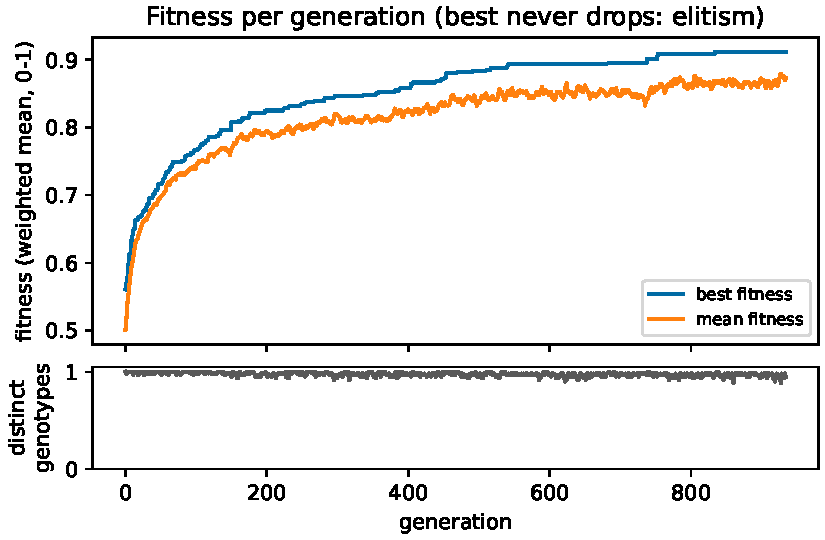
\includegraphics[width=\columnwidth]{figures/korobeiniki-s1-evolution.pdf}}
 \caption{Korobeiniki, seed 1. Top: best and mean fitness per generation. Elitism keeps the best curve non-decreasing. Bottom: share of distinct genotypes in the population.}
 \label{fig:evolution}
\end{figure}

\textbf{Is the GA needed?} Table~\ref{tab:experiments} compares five seeds with a random search
that scores as many random plans as the first GA run did (33,060 and 56,100 plans for the two folk tunes). Random search stays near 0.6 because it never finds coherent phrases (coherence 0), while every GA run on the folk tunes reaches 0.85 to 0.94. The seeds end on different plans: on average, 29\% (Ievan Polkka) and 38\%
(Korobeiniki) of the genes differ between two seeds. The same configuration therefore yields
different arrangements, as the assignment requires.

\begin{table}[t]
 \centering
 \footnotesize
 \setlength{\tabcolsep}{4pt}
 \begin{tabular}{@{}lccc@{}}
  \toprule
  & Ievan Polkka & Korobeiniki & 6 MIDI songs \\
  \midrule
  GA, mean of 5 seeds & 0.92 & 0.88 & 0.85 \\
  GA, worst seed & 0.90 & 0.85 & 0.79 \\
  Random search & 0.62 & 0.60 & 0.58 \\
  Genes differing & 29\% & 38\% & 41\% \\
  \midrule
  \multicolumn{4}{@{}l}{\emph{Ablation, seed 1: criterion score, weight 1 $\rightarrow$ 0}} \\
  coherence & 0.94 $\rightarrow$ 0.44 & 0.96 $\rightarrow$ 0.25 & 0.74 $\rightarrow$ 0.14 \\
  contrast & 1.00 $\rightarrow$ 0.52 & 0.75 $\rightarrow$ 0.56 & 0.82 $\rightarrow$ 0.47 \\
  bass smoothness & 0.99 $\rightarrow$ 0.60 & 1.00 $\rightarrow$ 0.77 & 0.95 $\rightarrow$ 0.65 \\
  idiom & 0.98 $\rightarrow$ 0.56 & 0.97 $\rightarrow$ 0.67 & 0.93 $\rightarrow$ 0.55 \\
  fidelity & 1.00 $\rightarrow$ 0.25 & 1.00 $\rightarrow$ 0.22 & 0.89 $\rightarrow$ 0.38 \\
  register & 1.00 $\rightarrow$ 0.87 & 1.00 $\rightarrow$ 0.99 & 0.94 $\rightarrow$ 0.82 \\
  complementarity & 0.63 $\rightarrow$ 0.61 & 0.75 $\rightarrow$ 0.73 & 0.71 $\rightarrow$ 0.63 \\
  \bottomrule
 \end{tabular}
 \caption{Fitness with the default weights. Random search scores as many plans as the first GA
 run; genes differing: mean share of genes that differ between two seeds. The MIDI column averages
 the six songs. Ablation: removing a criterion lowers its own score; on the two folk tunes,
 complementarity and register move least.}
 \label{tab:experiments}
\end{table}

\textbf{Ablation and hyperparameter variation.} Setting one weight to 0 lowers that criterion
(Table~\ref{tab:experiments}). Without fidelity, the GA moves most bars of the melody by an octave; without coherence, it changes
textures inside phrases; without contrast, the chorus loses its denser accompaniment. On the folk
tunes, complementarity is bounded by the busy melodies, and register drops only where P2 echoes
the melody or the melody moves down an octave. The submitted pieces vary the seed (samples
korobeiniki-s1 and korobeiniki-s2) and the contrast weight (ievan-polkka-s1 and
ievan-polkka-s1-contrast0). With
contrast at 0, the GA prefers a parallel line of chord tones under the melody instead of a held
verse and an arpeggiated chorus.

\textbf{Listening.} In Ievan Polkka (seed 1), the first A part holds the chord root over a walking
bass and a half-time beat, the B parts switch to fast arpeggios with a sixteenth-note beat, and a
snare fill closes every phrase. Korobeiniki keeps arpeggios throughout and saves the dense drums for the bridge (B), where the melody holds half notes. The noise channel sounds 39\% to 46\% of
the time, close to the 39\% measured in NES game music, but our P2 and TR channels never rest (100\%, against 84\% and 70\% in that corpus \cite{donahue2018nes}).

\textbf{MIDI songs.} We also arranged excerpts (32--56 bars) of six Brazilian songs from fan-made
MIDI files: \emph{Voa Voa} (Chiclete com Banana), \emph{Mulher de Fases} (Raimundos), \emph{Amor
I Love You} (Marisa Monte), \emph{Por Voc\^e} (Bar\~ao Vermelho), \emph{Aquarela} (Toquinho) and
\emph{Fico Assim Sem Voc\^e} (Adriana Calcanhotto).
In four files, the embedded lyric syllables identify the sung melody track; in the other two, the
melody is the monophonic line that plays throughout. The \emph{Voa Voa} file was recorded
live: it states 120 BPM, but its drum hits fit a sixteenth-note grid at 110.1 BPM (grid fit 0.90,
against 0.04 for the stated tempo), so the reader re-estimates the grid before cutting bars. These runs allow 4000 generations (stagnation window 200) and stopped after 800 to 3682. We repeated the experiments on every song (last column of
Table~\ref{tab:experiments}). The GA beats random search on each song (0.79--0.89 against
0.55--0.63), the seeds differ more (41\% of the genes), and removing a criterion lowers its own
score in at least five of the six songs, register and complementarity included. The songs score
lower than the folk tunes on average (0.85 against 0.90). Their melodies often sit in octaves 3--4,
so keeping the written register conflicts with keeping P2 below the melody (seed 1: fidelity
0.73--0.97, register 0.87--0.99), and coherence is lower (0.58--0.88, against 0.83--0.96 for the
folk tunes).

\section{Discussion and Future Work}\label{sec:discussion}

The experiments show that the search, not chance, produces the arrangements, but the approach has
clear limits. The fitness is a weighted mean of hand-written heuristics, a common choice whose weights are hard to tune \cite{fernandez2013ai} and that hides the conflicts between objectives. A Pareto front \cite{freitas2011melody,carpentier2010solving}
would expose these trade-offs. Automatic chord detection on MIDI songs is approximate, and we did not measure its errors. The textures come from a fixed vocabulary, so the GA chooses between
arranging gestures but does not invent new ones. The bass never rests, and P2 rests only where it follows the melody. Only 4/4 lead
sheets are supported. Our chip synthesizer uses one fixed duty cycle per pulse channel and no volume envelopes or pitch effects, and we do not use the chip's sample channel. Future work includes a fitness learned from the NES
Music Database \cite{donahue2018nes}, evolving rhythmic and melodic variations of the P2 and TR
lines, and a listening test with A/B comparisons, as in \cite{donahue2019lakhnes}.

\section{AI Usage Statement}

This work was developed with Claude Code (Anthropic) under the author's direction: brainstorming,
checking the design against the course material and the literature, writing the specification,
the code and its tests, transcribing the two lead sheets and drafting this text. The author chose
the method, the constraint and the songs, listened to the inputs and outputs, and reviewed the
results.

\bibliography{references}

\end{document}
